\subsection{Retourner la réponse textuelle sous la forme d'un signal audio}
Une fois une réponse générée, il ne reste plus qu'à la renvoyer à l'utilisateur sous une forme audio, ce qui est un autre calcul rapide qui peut accompli en temps réel. Cela est rendu possible avec le \gls{cnn} \texttt{Wavenet} de \cite{wavenet}. En effet, il est possible de générer n’importe quel ton de voix avec \texttt{Wavenet}, option qui pourrait être laissée à la discrétion de l’utilisateur. À titre d’exemple, cette architecture neurale est tellement puissante qu’il est possible de lui faire imiter la voix du président. Cette découverte récente par \textbf{Google} marquera donc la première occurrence d'une réplique parfaite du timbre d'une voix humaine réelle plutôt qu’une voix aux allures robotiques, ainsi l’illusion est bien réussie. La façon dont \texttt{Wavenet} fonctionne est d’établir un préalable statistique (une variable conditionnée) qui est donné à un premier algorithme qui s’occupe de trouver les bons tons de voix à générer avec \texttt{Wavenet}, à partir du texte. C’est ainsi que \texttt{Wavenet}, conditionné par le ton de voix demandé et par le texte fourni, peut générer la voix de façon réaliste. C’est une méthode point par point, où chaque point dans la vague audio est généré en fonction des points précédents et du conditionnement demandé. L'entraînement de ce réseau se fait à très bas niveau sur le signal qui est à un taux d’échantillonnage de 16 kHz, ce qui est suffisant pour capturer les infimes variations de quelqu’un qui parlerait réellement dans un enregistrement. Cette phase générative est illustrée dans la \autoref{fig:wavenet}.

\begin{figure*}
  \centering
  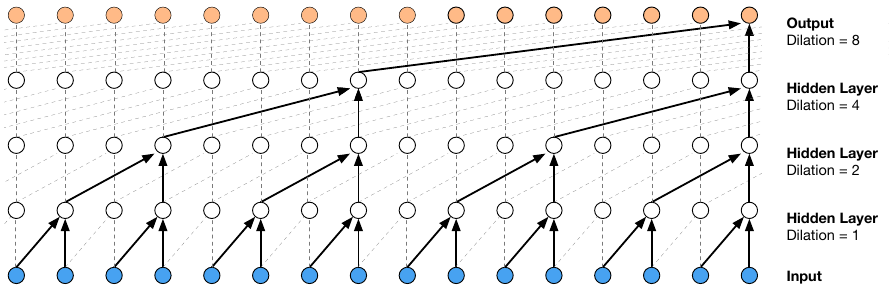
\includegraphics[width=\textwidth]{wavenet}
  \caption{À l’aide de convolutions causales dilatées, il est possible de prédire le prochain point dans la vague audio de façon efficace. Il s'agit d'un modèle autorégressif: les points passés sont utilisés pour prédire les points suivants du même signal. Ainsi, la sortie est remise en entrée pour le calcul de l’étape suivante, cet échantillonngage peut faire usage de mémoire cache, ce qui donne à cet algorithme un temps linéaire pour la génération dépendant de la longueur du signal à générer \cite{wavenet}.}
  \label{fig:wavenet}
\end{figure*}
